% ME 144L Dynamic Systems & Controls — Cheat Sheet
\documentclass[8pt,twocolumn]{article}

\usepackage[top=0.3in, bottom=0.3in, left=0.35in, right=0.35in]{geometry}
\usepackage{amsmath,amssymb}
\usepackage{booktabs,array}
\usepackage[table]{xcolor}
\usepackage{tikz}
\usetikzlibrary{arrows.meta}
\usepackage{multicol}
\usepackage{fancybox}

\definecolor{accent}{HTML}{BF5700}
\definecolor{bodytext}{HTML}{333333}
\definecolor{ansbg}{HTML}{FFFFFF}
\definecolor{ansframe}{HTML}{D9A87C}

\color{bodytext}
\pagestyle{empty}
\setlength{\parindent}{0pt}
\setlength{\parskip}{1.5pt}
\setlength{\columnsep}{10pt}
\setlength{\jot}{1pt}

\newcommand{\prob}[1]{%
  \vspace{3pt}%
  {\scriptsize\bfseries\textcolor{accent}{#1}}%
  \vspace{1pt}\par\noindent%
}
\newcommand{\partlabel}[1]{%
  \vspace{2pt}\noindent{\scriptsize\bfseries\textcolor{accent}{#1}}\par%
}
\newcommand{\stmtbegin}{\par\vspace{1pt}\begingroup\scriptsize\itshape%
  \textcolor{accent}{\vrule width 1.5pt}\hspace{3pt}%
  \begin{minipage}[t]{\dimexpr\columnwidth-5pt}}
\newcommand{\stmtend}{\end{minipage}\endgroup\par\vspace{1pt}}
\newcommand{\final}[1]{%
  \par\noindent\centerline{\fboxsep=2pt\fcolorbox{ansframe}{ansbg}{\footnotesize\textbf{#1}}}%
}
\newcommand{\finalrow}[1]{%
  \\\noalign{\centerline{\fboxsep=2pt\fcolorbox{ansframe}{ansbg}{\footnotesize\textbf{#1}}}}%
}
\newcommand{\finalbox}[1]{%
  \par\noindent\centerline{\fboxsep=2pt\fcolorbox{ansframe}{ansbg}{\parbox{0.88\columnwidth}{\footnotesize#1}}}%
  \par%
}

% Bond-graph TikZ shortcuts
\tikzset{
  jct/.style={circle, draw, inner sep=1.5pt, font=\tiny\bfseries},
  >=Stealth
}

\begin{document}
\scriptsize
\setlength{\abovedisplayskip}{1pt}
\setlength{\belowdisplayskip}{0pt}
\setlength{\abovedisplayshortskip}{0pt}
\setlength{\belowdisplayshortskip}{0pt}

% ═══════════════════════════════════════════════
% QUIZ PROBLEMS
% ═══════════════════════════════════════════════

\prob{Quiz -- \#1 -- Weighted \& Delayed Steps and Ramps}

\stmtbegin
Write expressions for each signal in terms of weighted and delayed unit steps $u_s$ and ramps $u_r$.
\stmtend

\partlabel{(a) Piecewise linear signal:}
Flat 0 for $t\in[0,1)$; ramp $+1$ at $t{=}1$; slope changes
$-\!\tfrac{1}{2}$ at $t{=}2,3,4,5$; $+1$ at $t{=}6$; $+2$ at $t{=}7$;
$-2$ at $t{=}8,9$.

\finalbox{$u = u_r(t{-}1) - \tfrac{1}{2}u_r(t{-}2)
- \tfrac{1}{2}u_r(t{-}3) - \tfrac{1}{2}u_r(t{-}4)
- \tfrac{1}{2}u_r(t{-}5)$\\[1pt]
$\quad + u_r(t{-}6) + 2\,u_r(t{-}7)
- 2\,u_r(t{-}8) - 2\,u_r(t{-}9)$}

\partlabel{(b) Signal with step and ramp components:}
Step up at $t{=}0$; ramp $-\!\tfrac{1}{2}$ at $t{=}2$;
$+\!\tfrac{1}{2}$ at $t{=}4,5$; step down at $t{=}4$;
$+\!\tfrac{3}{2}$ at $t{=}7$; $-2$ at $t{=}8$; step down at $t{=}9$.

\finalbox{$u = u_s(t) - \tfrac{1}{2}u_r(t{-}2)
+ \tfrac{1}{2}u_r(t{-}4) - u_s(t{-}4)
+ \tfrac{1}{2}u_r(t{-}5)$\\[1pt]
$\quad + \tfrac{3}{2}u_r(t{-}7) - 2\,u_r(t{-}8)
- 2\,u_s(t{-}9)$}

% ──────────────────────────────────────────────
\prob{Quiz -- \#2 -- 2nd Order System Damping Ratio Ranges}

\stmtbegin
$\ddot{y}+2\zeta\omega_n\dot{y}+\omega_n^2 y=u(t)$.
Identify $\zeta$ range for each step response plot.
\stmtend

Eigenvalues $\lambda=-\zeta\omega_n\pm\omega_n\sqrt{\zeta^2-1}$;
$\operatorname{Re}(\lambda)=-\zeta\omega_n$ governs decay/growth.

\begin{center}\scriptsize
\renewcommand{\arraystretch}{1.25}
\begin{tabular}{@{}lll@{}}
\toprule
\textbf{Plot} & \textbf{Behavior} & \textbf{$\zeta$ range} \\
\midrule
1 & Monotone, no overshoot & $\zeta\ge1$ (overdamped) \\
2 & Overshoot, decaying osc.\ & $0<\zeta<1$ (underdamped) \\
3 & Sustained oscillation & $\zeta=0$ (undamped) \\
4 & Growing oscillation & $-1<\zeta<0$ (neg.\ damped) \\
\bottomrule
\end{tabular}
\end{center}

% ──────────────────────────────────────────────
\prob{Quiz -- \#3 -- 2nd Order ODE: Homogeneous + Particular + Laplace}

\stmtbegin
$\ddot{y}+2\dot{y}+2y=u(t)$
\stmtend

\partlabel{(a-i)\; $u(t)=1$,\; $y(0)=1$,\; $\dot{y}(0)=0$}

\textbf{Homogeneous:} $y_h=ce^{\lambda t}$,
CE $\lambda^2+2\lambda+2=0$:
\[
\lambda=\tfrac{-2\pm\sqrt{4-8}}{2}=-1\pm j
\qquad(\alpha{=}{-1},\;\omega{=}1)
\]
$y_h=e^{-t}(C_1\cos t+C_2\sin t)$

\textbf{Particular:} constant $\Rightarrow y_p=K$;\;
$2K=1\Rightarrow y_p=\tfrac{1}{2}$

\textbf{Full:} $y=e^{-t}(C_1\cos t+C_2\sin t)+\tfrac{1}{2}$

ICs:\; $y(0){=}1$: $C_1+\tfrac{1}{2}=1\Rightarrow C_1=\tfrac{1}{2}$\\
$\dot{y}(0){=}0$: $-C_1+C_2=0\Rightarrow C_2=\tfrac{1}{2}$

\final{$y(t)=e^{-t}\!\bigl(\tfrac{1}{2}\cos t+\tfrac{1}{2}\sin t\bigr)+\tfrac{1}{2}$}

\partlabel{(a-ii)\; $u(t)=11\cos 2t$,\; $y(0)=0$,\; $\dot{y}(0)=0$}

\textbf{Homogeneous:} same $y_h=e^{-t}(C_1\cos t+C_2\sin t)$

\textbf{Particular:} $y_p=K_1\cos 2t+K_2\sin 2t$
\begin{align*}
\dot{y}_p &= -2K_1\sin 2t+2K_2\cos 2t \\
\ddot{y}_p &= -4K_1\cos 2t-4K_2\sin 2t
\end{align*}
Substitute, collect:
\begin{align*}
\cos 2t&:\; {-4K_1+4K_2+2K_1}=11 \;\Rightarrow\; {-2K_1+4K_2=11} \\
\sin 2t&:\; {-4K_2-4K_1+2K_2}=0 \;\Rightarrow\; {-4K_1-2K_2=0}
\end{align*}
$K_2=-2K_1$.\; $-2K_1-8K_1=11\Rightarrow K_1=-1.1$,\; $K_2=2.2$

\textbf{Full:}
$y=e^{-t}(C_1\cos t+C_2\sin t)-1.1\cos 2t+2.2\sin 2t$

ICs:\; $y(0){=}0$: $C_1-1.1=0 \Rightarrow C_1=1.1$\\
$\dot{y}(0){=}0$: $-C_1+C_2+4.4=0 \Rightarrow C_2=-3.3$

\final{$y(t)=e^{-t}(1.1\cos t-3.3\sin t)-1.1\cos 2t+2.2\sin 2t$}

\partlabel{(b) Stability:}
$\lambda=-1\pm j\;\Rightarrow\;\operatorname{Re}(\lambda)=-1<0$
\final{Stable --- both eigenvalues have negative real part}

\partlabel{(c) Laplace method for (a-i): $u(t)=1$, $y(0)=1$, $\dot{y}(0)=0$}

$\mathcal{L}\{\text{ODE}\}$:
$[s^2Y-s]+2[sY-1]+2Y=\tfrac{1}{s}$
\[
Y(s^2{+}2s{+}2)=\tfrac{1}{s}+s+2
\;\Rightarrow\;
Y=\frac{s^2+2s+1}{s(s^2+2s+2)}=\frac{(s{+}1)^2}{s[(s{+}1)^2+1]}
\]

PFD: $Y=\dfrac{A}{s}+\dfrac{\alpha s+\beta}{s^2+2s+2}$.\;
$A\!=\!\tfrac{1}{2}$, match: $\alpha\!=\!\tfrac{1}{2}$, $\beta\!=\!1$.
\[
Y=\frac{1}{2s}+\frac{1}{2}\!\cdot\!\frac{s+1}{(s{+}1)^2+1}
+\frac{1}{2}\!\cdot\!\frac{1}{(s{+}1)^2+1}
\]

\final{$y(t)=\tfrac{1}{2}+\tfrac{1}{2}e^{-t}\cos t+\tfrac{1}{2}e^{-t}\sin t$}

\partlabel{(d) Critically damped ($u=0$):}
Need repeated real roots: $(2\zeta\omega_n)^2=4\omega_n^2$.
Currently $\omega_n^2=2$, so need $\omega_n^2=1$.
\final{$\ddot{y}+2\dot{y}+y=0\;\Rightarrow\;\lambda=-1$ (repeated)}

% ═══════════════════════════════════════════════
% HW4 PROBLEMS
% ═══════════════════════════════════════════════

\prob{HW4 -- \#1 -- Signal Decomposition: Steps (8.2a) and Ramps (8.2b)}

\stmtbegin
Decompose signals into weighted/delayed steps and ramps.
\stmtend

\partlabel{(a) Rectangular pulse signal:}
Step up $t{=}0$, down $t{=}1$, down $t{=}2$, up $t{=}3$.
\final{$u(t)=u_s(t)-u_s(t{-}1)-u_s(t{-}2)+u_s(t{-}3)$}

\partlabel{(b) Triangular ramp signal:}
Ramp $+1$ at $t{=}1$, change $-2$ at $t{=}2$, $+1$ at $t{=}3$.
\final{$u(t)=u_r(t{-}1)-2\,u_r(t{-}2)+u_r(t{-}3)$}

% ──────────────────────────────────────────────
\prob{HW4 -- \#2 -- Repeated Roots: Homogeneous Solution (8.9c)}

\stmtbegin
$\ddot{y}+6\dot{y}+9y=0$,\; $y(0)=1$, $\dot{y}(0)=0$
\stmtend

CE: $\lambda^2+6\lambda+9=(\lambda+3)^2=0\;\Rightarrow\;\lambda_{1,2}=-3$ (repeated)

$y=C_1e^{-3t}+C_2\,te^{-3t}$

$y(0){=}1$: $C_1=1$.\quad
$\dot{y}(0){=}0$: $-3C_1+C_2=0\Rightarrow C_2=3$.

\final{$y(t)=e^{-3t}+3\,te^{-3t}$}

% ──────────────────────────────────────────────
\prob{HW4 -- \#3 -- Euler Identity \& Particular Solution (8.11)}

\stmtbegin
$\dot{y}+y=6e^{-2t}\cos 4t$
\stmtend

$y_p=e^{-2t}(K_1\cos 4t+K_2\sin 4t)$

$\dot{y}_p=e^{-2t}[(-2K_1{+}4K_2)\cos 4t+(-4K_1{-}2K_2)\sin 4t]$

Sub into $\dot{y}+y=6e^{-2t}\cos 4t$, divide by $e^{-2t}$:
\begin{align*}
\cos 4t&:\; -K_1+4K_2=6 \\
\sin 4t&:\; -4K_1-K_2=0 \;\Rightarrow\; K_2=-4K_1
\end{align*}
$-K_1-16K_1=6\Rightarrow K_1=-\tfrac{6}{17}$,\; $K_2=\tfrac{24}{17}$

\final{$y_p=e^{-2t}\!\left(\tfrac{24}{17}\sin 4t-\tfrac{6}{17}\cos 4t\right)$}

% ──────────────────────────────────────────────
\prob{HW4 -- \#4 -- Sinusoidal Particular Solution (8.12)}

\stmtbegin
$\ddot{y}+9\dot{y}+20y=5\sin 2t$
\stmtend

$y_p=K_1\cos 2t+K_2\sin 2t$,\;
$\dot{y}_p=-2K_1\sin 2t+2K_2\cos 2t$,\;
$\ddot{y}_p=-4K_1\cos 2t-4K_2\sin 2t$

Substitute:
\begin{align*}
\cos 2t&:\; 16K_1+18K_2=0 \\
\sin 2t&:\; -18K_1+16K_2=5
\end{align*}
$K_1=-\tfrac{9}{8}K_2$.\;
$\tfrac{162}{8}K_2+16K_2=\tfrac{290}{8}K_2=5
\Rightarrow K_2=\tfrac{4}{29}$,\; $K_1=-\tfrac{9}{58}$

\final{$y_p=-\tfrac{9}{58}\cos 2t+\tfrac{4}{29}\sin 2t$}

% ──────────────────────────────────────────────
\prob{HW4 -- \#5 -- Stability via Eigenvalue Analysis (8.18b)}

\stmtbegin
$\ddot{y}+\dot{y}-ay=0$.\; Find values of $a$ for stability.
\stmtend

CE: $\lambda^2+\lambda-a=0\;\Rightarrow\;
\lambda_{1,2}=\dfrac{-1\pm\sqrt{1+4a}}{2}$

\textbf{Case 1:} $1{+}4a<0$ ($a<-\!\tfrac{1}{4}$):
complex roots, $\operatorname{Re}(\lambda)=-\!\tfrac{1}{2}<0$ $\to$ stable.

\textbf{Case 2:} $1{+}4a\ge0$ ($a\ge-\!\tfrac{1}{4}$):
real roots. $\lambda_1=\tfrac{-1+\sqrt{1+4a}}{2}<0
\Rightarrow\sqrt{1+4a}<1\Rightarrow a<0$.

\final{Stable iff $a<0$;\quad marginal: $a{=}0$;\quad unstable: $a>0$}

% ═══════════════════════════════════════════════
% HW5 PROBLEMS
% ═══════════════════════════════════════════════

\prob{HW5 -- \#1 -- RC Circuit: State Equation \& Time Constant (9.4)}

\stmtbegin
Voltage source $V_s$, resistors $R_1$, $R_2$, capacitor $C$.
Derive state equation, time constant, and limiting cases.
\stmtend

\begin{center}
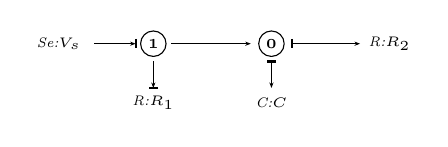
\begin{tikzpicture}[scale=0.75, every node/.style={font=\tiny}]
  \node[font=\tiny\itshape] (Se) at (-1.6,0) {Se:$V_s$};
  \node[jct] (j1) at (0,0) {1};
  \node[jct] (j0) at (2,0) {0};
  \node[font=\tiny\itshape] (R2) at (4,0) {R:$R_2$};
  \node[font=\tiny\itshape] (R1) at (0,-1) {R:$R_1$};
  \node[font=\tiny\itshape] (C)  at (2,-1) {C:$C$};
  % bonds
  \draw[-{Stealth[length=2pt]}] (-1.0,0)--(-0.3,0);
  \draw[-{Stealth[length=2pt]}] (0.3,0)--(1.65,0);
  \draw[-{Stealth[length=2pt]}] (2.35,0)--(3.5,0);
  \draw[-{Stealth[length=2pt]}] (0,-0.3)--(0,-0.75);
  \draw[-{Stealth[length=2pt]}] (2,-0.3)--(2,-0.75);
  % causality strokes
  \draw[thick] (-0.3,0.08)--(-0.3,-0.08);
  \draw[thick] (2.35,0.08)--(2.35,-0.08);
  \draw[thick] (0.08,-0.75)--(-0.08,-0.75);
  \draw[thick] (2.08,-0.3)--(1.92,-0.3);
\end{tikzpicture}
\end{center}

State eq.\ ($q_c$ = charge on $C$):
\[
\dot{q}_c = \frac{V_s}{R_1}
  -\frac{R_1+R_2}{R_1 R_2 C}\,q_c
\]

Standard form: $\dfrac{CR_1R_2}{R_1{+}R_2}\,\dot{q}_c + q_c
= \dfrac{CR_2}{R_1{+}R_2}\,V_s$

\partlabel{(b) Time constant:}
$\tau = \dfrac{CR_1R_2}{R_1+R_2}$.\;
$R_1{=}R_2{=}R{=}10\,\Omega$, $C{=}10^{-6}$\,F:
\final{$\tau = CR/2 = 5\times10^{-6}$ s}

\partlabel{(c) $R_2\to\infty$:}
$\tau\to CR_1$.\; Series $R_1$--$C$: $CR_1\dot{q}_c+q_c=CV_s$.

\partlabel{(d) $R_1\to0$:}
$\tau\to 0$.\; $q_c=CV_s$ (instantaneous tracking).

% ──────────────────────────────────────────────
\prob{HW5 -- \#2 -- Clutch-Spring: ODE \& Step Response (9.6c)}

\stmtbegin
Rotational spring $K_r$, damper $B_r$, input shaft $\Omega_s$.
\stmtend

\begin{center}
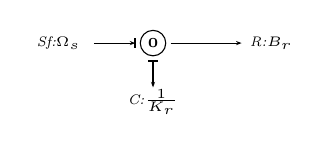
\begin{tikzpicture}[scale=0.75, every node/.style={font=\tiny}]
  \node[font=\tiny\itshape] (Sf) at (-1.6,0) {Sf:$\Omega_s$};
  \node[jct] (j0) at (0,0) {0};
  \node[font=\tiny\itshape] (Br) at (2,0) {R:$B_r$};
  \node[font=\tiny\itshape] (Kr) at (0,-1) {C:$\frac{1}{K_r}$};
  \draw[-{Stealth[length=2pt]}] (-1.0,0)--(-0.3,0);
  \draw[-{Stealth[length=2pt]}] (0.3,0)--(1.5,0);
  \draw[-{Stealth[length=2pt]}] (0,-0.3)--(0,-0.75);
  % causality
  \draw[thick] (-0.3,0.08)--(-0.3,-0.08);
  \draw[thick] (0.08,-0.3)--(-0.08,-0.3);
\end{tikzpicture}
\end{center}

ODE in torque $T_K=K_r\theta_K$:\;
$\dfrac{B_r}{K_r}\dot{T}_K + T_K = B_r\,\Omega_s(t)$

Step response ($\Omega_s=(\Omega_s)_0$, zero IC):
\final{$T_K(t) = B_r(\Omega_s)_0\!\left[1-e^{-K_r t/B_r}\right]$}

Steady state at $t=4\tau=\dfrac{4B_r}{K_r}$.

% ──────────────────────────────────────────────
\prob{HW5 -- \#3 -- Parachutist: Switching Dynamics (9.12)}

\stmtbegin
Mass $m$, drag $B$ (small chute), $10B$ (both chutes).
\stmtend

\begin{center}
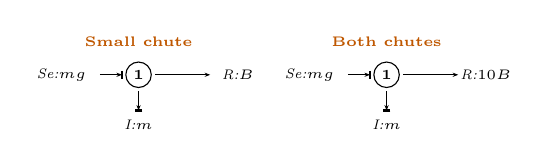
\begin{tikzpicture}[scale=0.7, every node/.style={font=\tiny}]
  % Small chute
  \node[font=\tiny\bfseries\color{accent}] at (0,0.6) {Small chute};
  \node[font=\tiny\itshape] (Se1) at (-1.4,0) {Se:$mg$};
  \node[jct] (j1a) at (0,0) {1};
  \node[font=\tiny\itshape] (B1) at (1.8,0) {R:$B$};
  \node[font=\tiny\itshape] (I1) at (0,-0.9) {I:$m$};
  \draw[-{Stealth[length=2pt]}] (-0.7,0)--(-0.3,0);
  \draw[-{Stealth[length=2pt]}] (0.3,0)--(1.3,0);
  \draw[-{Stealth[length=2pt]}] (0,-0.3)--(0,-0.65);
  \draw[thick] (-0.3,0.07)--(-0.3,-0.07);
  \draw[thick] (0.07,-0.65)--(-0.07,-0.65);
  % Both chutes
  \begin{scope}[xshift=4.5cm]
  \node[font=\tiny\bfseries\color{accent}] at (0,0.6) {Both chutes};
  \node[font=\tiny\itshape] (Se2) at (-1.4,0) {Se:$mg$};
  \node[jct] (j1b) at (0,0) {1};
  \node[font=\tiny\itshape] (B2) at (1.8,0) {R:$10B$};
  \node[font=\tiny\itshape] (I2) at (0,-0.9) {I:$m$};
  \draw[-{Stealth[length=2pt]}] (-0.7,0)--(-0.3,0);
  \draw[-{Stealth[length=2pt]}] (0.3,0)--(1.3,0);
  \draw[-{Stealth[length=2pt]}] (0,-0.3)--(0,-0.65);
  \draw[thick] (-0.3,0.07)--(-0.3,-0.07);
  \draw[thick] (0.07,-0.65)--(-0.07,-0.65);
  \end{scope}
\end{tikzpicture}
\end{center}

ODEs:\;
Small: $\dfrac{m}{B}\dot{V}+V=\dfrac{mg}{B}$\qquad
Both: $\dfrac{m}{10B}\dot{V}+V=\dfrac{mg}{10B}$

\partlabel{(b) Velocity response:}
Phase 1 ($0<t<4m/B$, $\tau_1=m/B$):
\[
v(t)=\frac{mg}{B}\!\left[1-e^{-Bt/m}\right]
\;\xrightarrow{t\to4\tau_1}\;
V\approx\frac{0.98\,mg}{B}
\]
Phase 2 ($t>4m/B$, $\hat{t}=t-4m/B$, $\tau_2=m/(10B)$):
\[
V(t)=\frac{mg}{10B}+\frac{9mg}{10B}\,e^{-10B\hat{t}/m}
\]
Terminal $V\to mg/(10B)$ reached at $t\approx4.4\,m/B$.

\partlabel{(c) Force on skydiver $F_m=m\dot{v}$:}

Phase 1: $F_m = mg\,e^{-t/\tau_1}$,\; $\tau_1=m/B$

Phase 2: $F_m = -9mg\,e^{-\hat{t}/\tau_2}$,\; $\tau_2=m/(10B)$

% ──────────────────────────────────────────────
\prob{HW5 -- \#4 -- Spring-Mass-Damper: $\omega_n$, $\eta$, Min Damping (9.23)}

\stmtbegin
$M{=}320$\,kg, $K_{eq}{=}16000$\,N/m (4 springs $\times$ 4000),
$B_{eq}{=}1200$\,Ns/m.
\stmtend

\begin{center}
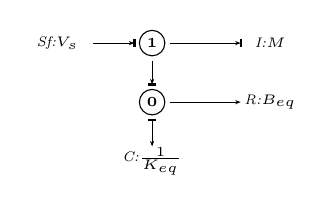
\begin{tikzpicture}[scale=0.75, every node/.style={font=\tiny}]
  \node[font=\tiny\itshape] (Sf) at (-1.6,0) {Sf:$V_s$};
  \node[jct] (j1) at (0,0) {1};
  \node[font=\tiny\itshape] (IM) at (2,0) {I:$M$};
  \node[jct] (j0) at (0,-1) {0};
  \node[font=\tiny\itshape] (Rb) at (2,-1) {R:$B_{eq}$};
  \node[font=\tiny\itshape] (Ck) at (0,-2) {C:$\frac{1}{K_{eq}}$};
  \draw[-{Stealth[length=2pt]}] (-1.0,0)--(-0.3,0);
  \draw[-{Stealth[length=2pt]}] (0.3,0)--(1.5,0);
  \draw[-{Stealth[length=2pt]}] (0,-0.3)--(0,-0.7);
  \draw[-{Stealth[length=2pt]}] (0.3,-1)--(1.5,-1);
  \draw[-{Stealth[length=2pt]}] (0,-1.3)--(0,-1.75);
  % causality
  \draw[thick] (-0.3,0.07)--(-0.3,-0.07);
  \draw[thick] (1.5,0.07)--(1.5,-0.07);
  \draw[thick] (0.07,-0.7)--(-0.07,-0.7);
  \draw[thick] (0.07,-1.3)--(-0.07,-1.3);
\end{tikzpicture}
\end{center}

State equations ($P{=}MV_M$, $X{=}$spring deflection):
\[
\left[\begin{smallmatrix}\dot{P}\\\dot{X}\end{smallmatrix}\right]=
\left[\begin{smallmatrix}-B_{eq}/M & K_{eq}\\
-1/M & 0\end{smallmatrix}\right]
\left[\begin{smallmatrix}P\\X\end{smallmatrix}\right]+
\left[\begin{smallmatrix}B_{eq}\\1\end{smallmatrix}\right]V_s
\]

2nd-order ODE:
$\ddot{P}+\dfrac{B_{eq}}{M}\dot{P}+\dfrac{K_{eq}}{M}P
=B_{eq}\dot{V}_s+K_{eq}V_s$

$\omega_n=\sqrt{\dfrac{K_{eq}}{M}}
=\sqrt{\dfrac{16000}{320}}=5\sqrt{2}\approx7.07\;\text{rad/s}$

$\eta=\dfrac{B_{eq}}{2\sqrt{K_{eq}M}}
=\dfrac{1200}{2\sqrt{16000\!\cdot\!320}}
=\dfrac{1200}{4525.5}\approx0.265$

\final{Underdamped ($\eta<1$)}

\partlabel{(b) Min $B$ per shock for no oscillation ($\eta\ge1$):}
$4B_{\min}=2\sqrt{K_{eq}M}$\;\;$\Rightarrow$\;\;
$B_{\min}=\sqrt{K M}=\sqrt{4000\!\cdot\!320}$

\final{$B_{\min}=800\sqrt{2}\;\text{Ns/m}$}

% ──────────────────────────────────────────────
\prob{HW5 -- \#5 -- Pumping Station: Bond Graph, State Eqs, $\omega_n$, $\eta$ (9.25)}

\stmtbegin
Pump $P(t)$, pipe inertance $I$, tank capacitance $C$, valve $R$.
\stmtend

\begin{center}
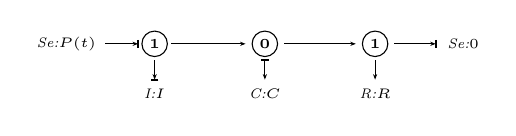
\begin{tikzpicture}[scale=0.7, every node/.style={font=\tiny}]
  \node[font=\tiny\itshape] (Se1) at (-1.6,0) {Se:$P(t)$};
  \node[jct] (j1a) at (0,0) {1};
  \node[jct] (j0)  at (2,0) {0};
  \node[jct] (j1b) at (4,0) {1};
  \node[font=\tiny\itshape] (Se2) at (5.6,0) {Se:$0$};
  \node[font=\tiny\itshape] (I)  at (0,-0.9) {I:$I$};
  \node[font=\tiny\itshape] (C)  at (2,-0.9) {C:$C$};
  \node[font=\tiny\itshape] (R)  at (4,-0.9) {R:$R$};
  % bonds
  \draw[-{Stealth[length=2pt]}] (-0.9,0)--(-0.3,0);
  \draw[-{Stealth[length=2pt]}] (0.3,0)--(1.65,0);
  \draw[-{Stealth[length=2pt]}] (2.35,0)--(3.65,0);
  \draw[-{Stealth[length=2pt]}] (4.35,0)--(5.1,0);
  \draw[-{Stealth[length=2pt]}] (0,-0.3)--(0,-0.65);
  \draw[-{Stealth[length=2pt]}] (2,-0.3)--(2,-0.65);
  \draw[-{Stealth[length=2pt]}] (4,-0.3)--(4,-0.65);
  % causality
  \draw[thick] (-0.3,0.07)--(-0.3,-0.07);
  \draw[thick] (0.07,-0.65)--(-0.07,-0.65);
  \draw[thick] (2.07,-0.3)--(1.93,-0.3);
  \draw[thick] (5.1,0.07)--(5.1,-0.07);
\end{tikzpicture}
\end{center}

State vars: $\Gamma$ (pipe momentum), $U_C$ (tank volume).
\[
\left[\begin{smallmatrix}\dot{\Gamma}\\\dot{U}_C\end{smallmatrix}\right]=
\left[\begin{smallmatrix}0 & -1/C\\
1/I & -1/(CR)\end{smallmatrix}\right]
\left[\begin{smallmatrix}\Gamma\\U_C\end{smallmatrix}\right]+
\left[\begin{smallmatrix}1\\0\end{smallmatrix}\right]P(t)
\]

\partlabel{(b) 2nd-order ODE for $Q_R=U_C/(CR)$:}
\[
\ddot{U}_C+\frac{1}{CR}\dot{U}_C+\frac{1}{CI}U_C=\frac{P(t)}{I}
\]

$\omega_n=\dfrac{1}{\sqrt{CI}}\,,\qquad
\eta=\dfrac{1}{2R}\sqrt{\dfrac{I}{C}}$

\partlabel{(c) Effect of $R$: $I/C=2$.}
$\eta=\dfrac{\sqrt{2}}{2R}$

\begin{center}\scriptsize
\renewcommand{\arraystretch}{1.2}
\begin{tabular}{@{}lcl@{}}
\toprule
$R$ & $\eta$ & Behavior \\
\midrule
$0.5$ & $\sqrt{2}\approx1.41$ & Overdamped \\
$2$ & $\sqrt{2}/4\approx0.35$ & Underdamped \\
\bottomrule
\end{tabular}
\end{center}

\finalbox{System changes from \textbf{overdamped} ($R{=}0.5$) to
\textbf{underdamped} ($R{=}2$).\\[1pt]
No overshoot requires $\eta\ge1\;\Rightarrow\;
R\le\frac{1}{2}\sqrt{I/C}$.}

\end{document}
